\section{Conlusions and Future Work}

\begin{frame}{Conclusion}
  \framesubtitle{Let's discuss the results}
  \begin{itemize}
    \item TinyViT proves that \textbf{transformer based models} can be efficient with fewer resources.
    \item Outperforms CNNs on \textbf{smaller datasets} like CIFAR-10 and CIFAR-100.
    \item \textbf{Requires improvements} for larger images like STL-10.
  \end{itemize}
\end{frame}

\begin{frame}[fragile]{Future Work}
  \framesubtitle{How can we improve ?}
  \begin{columns}
    \begin{column}{0.7\textwidth}
      \begin{itemize}
        \item Implement TinyViT for \textbf{Object Detection} (\textit{DETR}) and \textbf{Segmentation} (\textit{Segmenter}).
        \item Experiment with different \textbf{hyperparameters} (\textit{layers, embedding size, attention heads}).
        \item Explore pretraining on \textbf{larger datasets} to improve performance.
      \end{itemize}
    \end{column}
    \begin{column}{0.3\textwidth}
      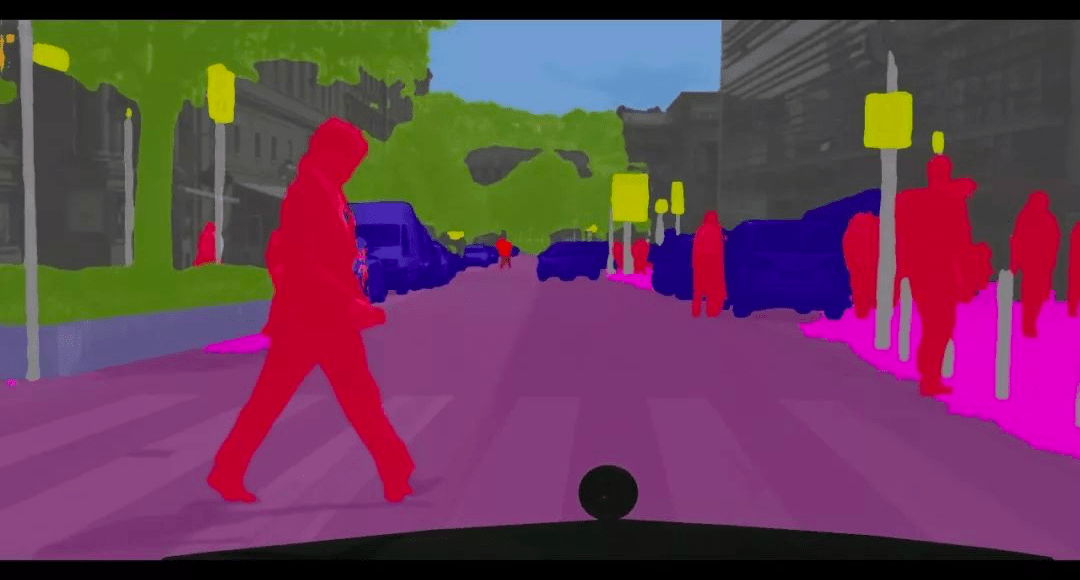
\includegraphics[width=\textwidth]{images/segmentation.png}
      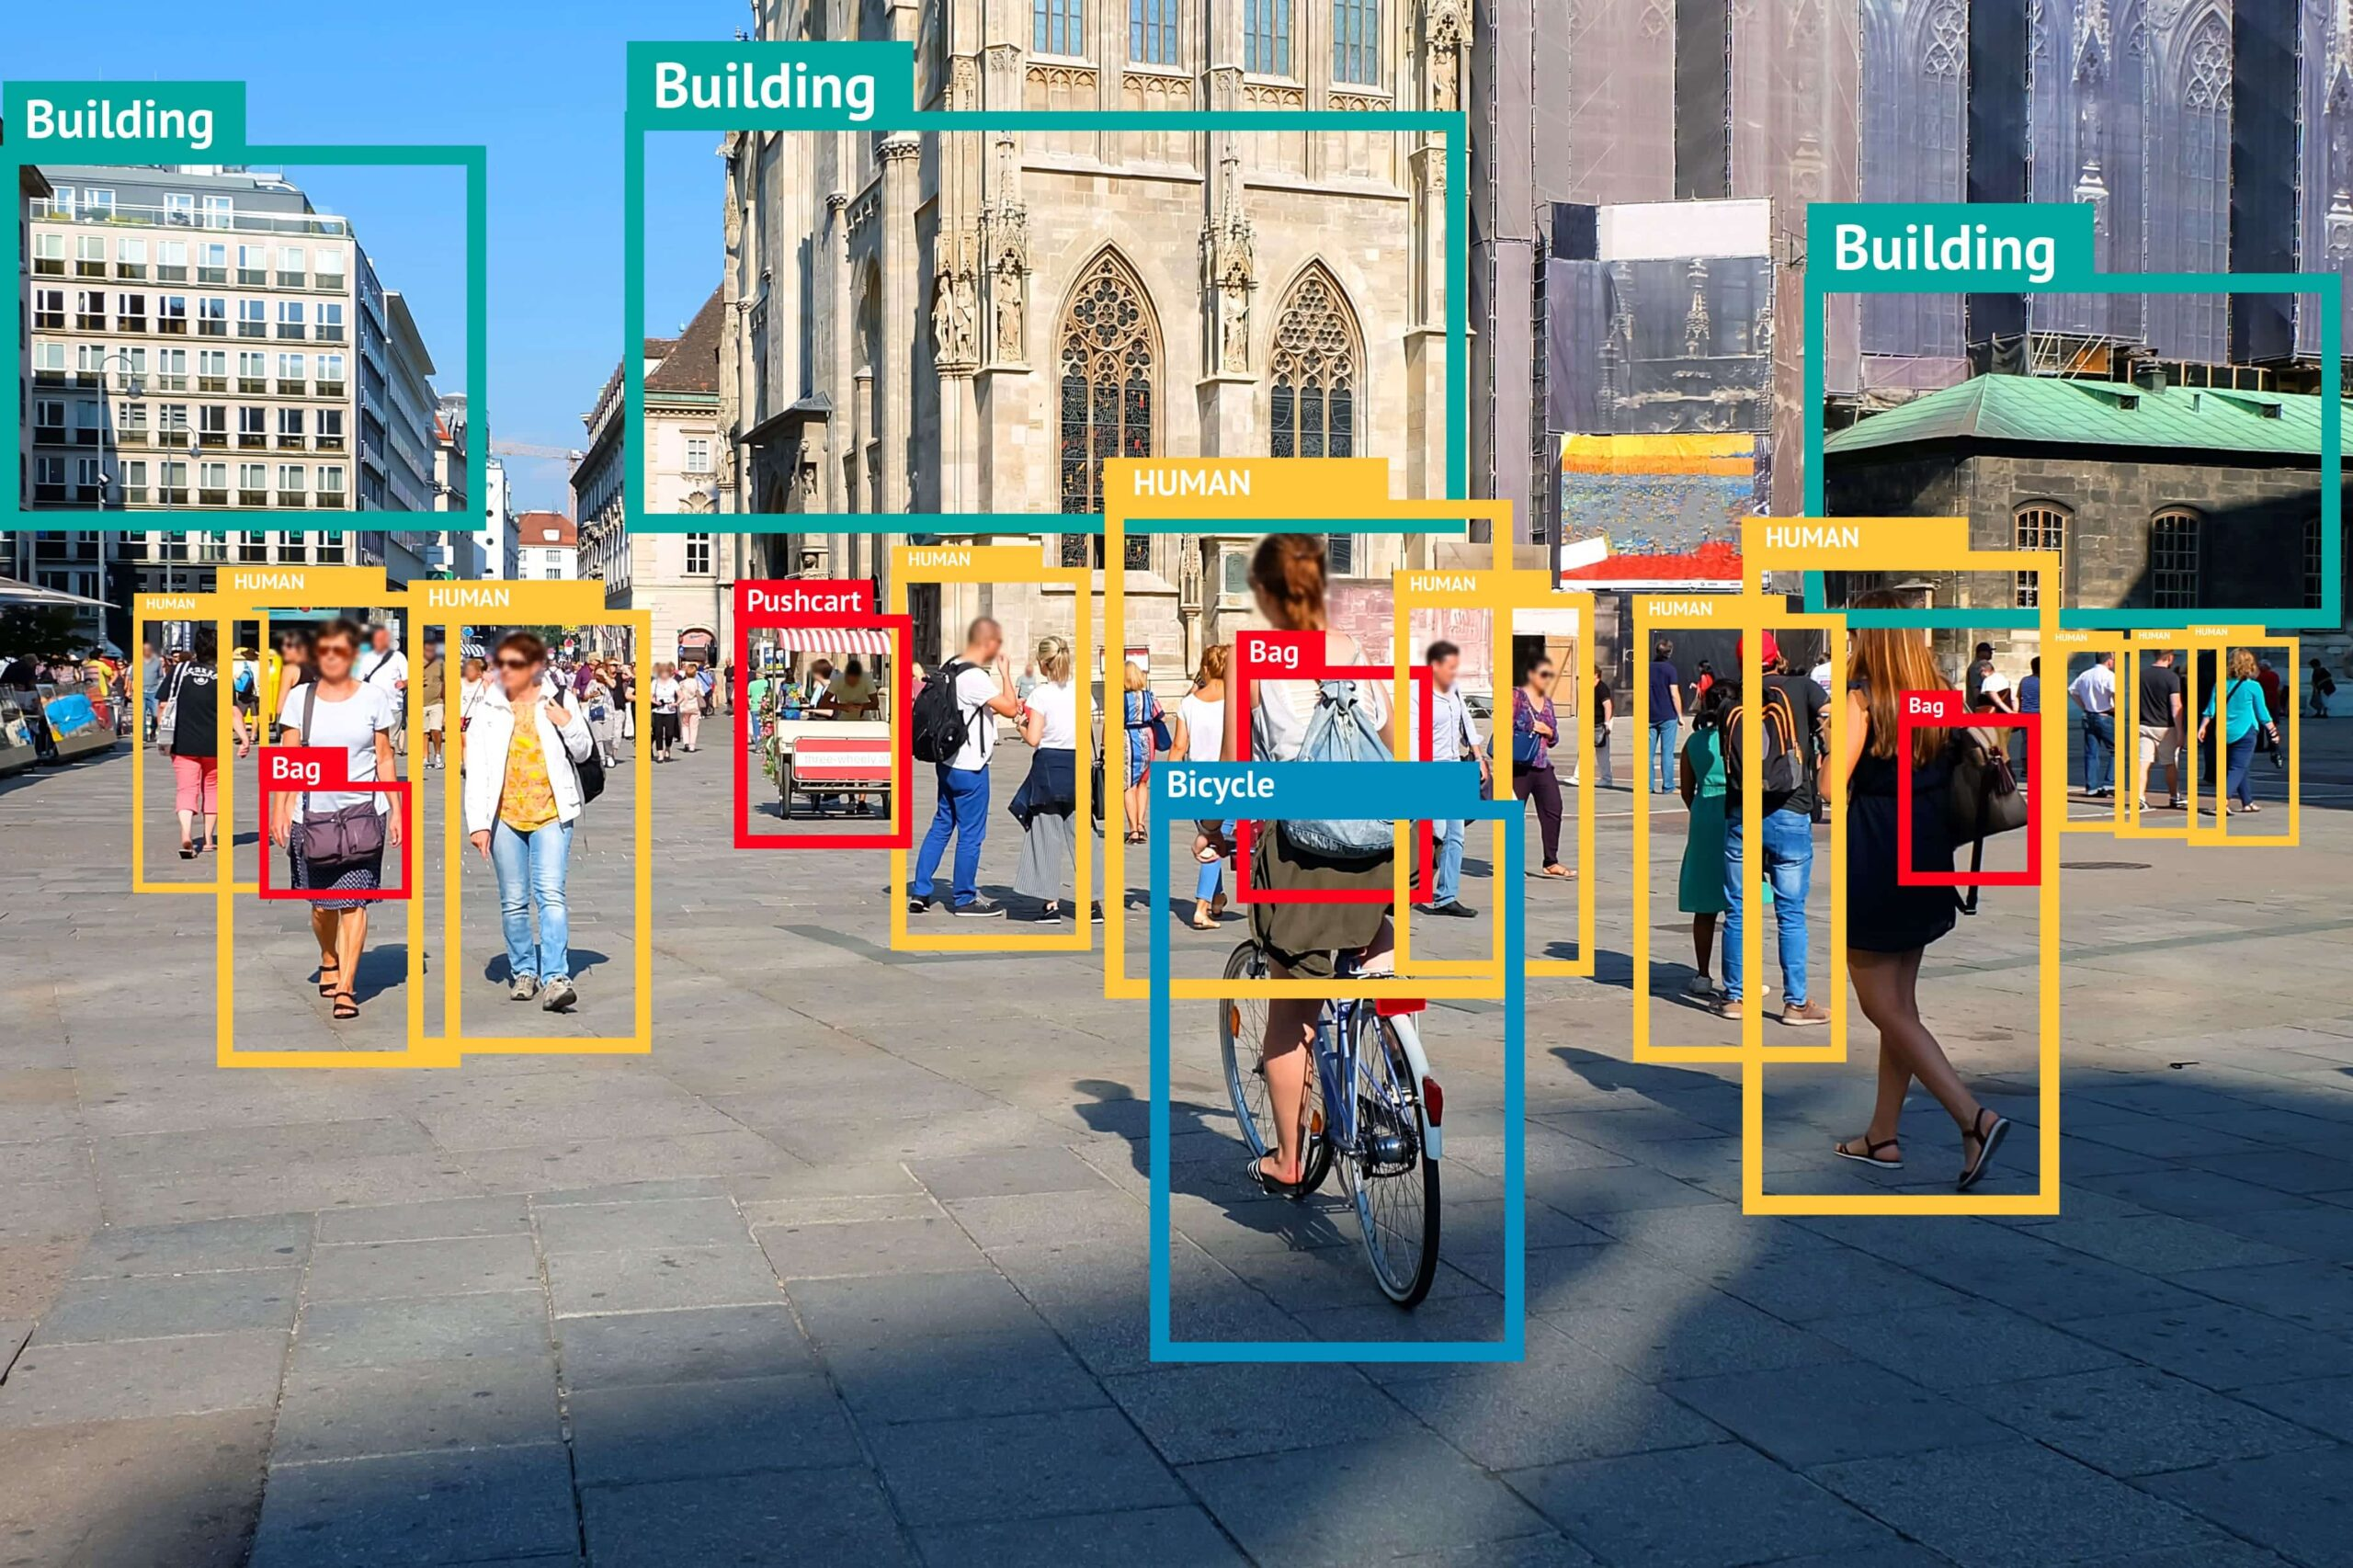
\includegraphics[width=\textwidth]{images/objectdetection.jpg}
    \end{column}
  \end{columns}
\end{frame}